\documentclass[]{article}
\usepackage{lmodern}
\usepackage{amssymb,amsmath}
\usepackage{ifxetex,ifluatex}
\usepackage{fixltx2e} % provides \textsubscript
\ifnum 0\ifxetex 1\fi\ifluatex 1\fi=0 % if pdftex
  \usepackage[T1]{fontenc}
  \usepackage[utf8]{inputenc}
\else % if luatex or xelatex
  \ifxetex
    \usepackage{mathspec}
  \else
    \usepackage{fontspec}
  \fi
  \defaultfontfeatures{Ligatures=TeX,Scale=MatchLowercase}
\fi
% use upquote if available, for straight quotes in verbatim environments
\IfFileExists{upquote.sty}{\usepackage{upquote}}{}
% use microtype if available
\IfFileExists{microtype.sty}{%
\usepackage{microtype}
\UseMicrotypeSet[protrusion]{basicmath} % disable protrusion for tt fonts
}{}
\usepackage[margin=1in]{geometry}
\usepackage{hyperref}
\hypersetup{unicode=true,
            pdftitle={Lab 1},
            pdfauthor={qy2205},
            pdfborder={0 0 0},
            breaklinks=true}
\urlstyle{same}  % don't use monospace font for urls
\usepackage{color}
\usepackage{fancyvrb}
\newcommand{\VerbBar}{|}
\newcommand{\VERB}{\Verb[commandchars=\\\{\}]}
\DefineVerbatimEnvironment{Highlighting}{Verbatim}{commandchars=\\\{\}}
% Add ',fontsize=\small' for more characters per line
\usepackage{framed}
\definecolor{shadecolor}{RGB}{248,248,248}
\newenvironment{Shaded}{\begin{snugshade}}{\end{snugshade}}
\newcommand{\KeywordTok}[1]{\textcolor[rgb]{0.13,0.29,0.53}{\textbf{#1}}}
\newcommand{\DataTypeTok}[1]{\textcolor[rgb]{0.13,0.29,0.53}{#1}}
\newcommand{\DecValTok}[1]{\textcolor[rgb]{0.00,0.00,0.81}{#1}}
\newcommand{\BaseNTok}[1]{\textcolor[rgb]{0.00,0.00,0.81}{#1}}
\newcommand{\FloatTok}[1]{\textcolor[rgb]{0.00,0.00,0.81}{#1}}
\newcommand{\ConstantTok}[1]{\textcolor[rgb]{0.00,0.00,0.00}{#1}}
\newcommand{\CharTok}[1]{\textcolor[rgb]{0.31,0.60,0.02}{#1}}
\newcommand{\SpecialCharTok}[1]{\textcolor[rgb]{0.00,0.00,0.00}{#1}}
\newcommand{\StringTok}[1]{\textcolor[rgb]{0.31,0.60,0.02}{#1}}
\newcommand{\VerbatimStringTok}[1]{\textcolor[rgb]{0.31,0.60,0.02}{#1}}
\newcommand{\SpecialStringTok}[1]{\textcolor[rgb]{0.31,0.60,0.02}{#1}}
\newcommand{\ImportTok}[1]{#1}
\newcommand{\CommentTok}[1]{\textcolor[rgb]{0.56,0.35,0.01}{\textit{#1}}}
\newcommand{\DocumentationTok}[1]{\textcolor[rgb]{0.56,0.35,0.01}{\textbf{\textit{#1}}}}
\newcommand{\AnnotationTok}[1]{\textcolor[rgb]{0.56,0.35,0.01}{\textbf{\textit{#1}}}}
\newcommand{\CommentVarTok}[1]{\textcolor[rgb]{0.56,0.35,0.01}{\textbf{\textit{#1}}}}
\newcommand{\OtherTok}[1]{\textcolor[rgb]{0.56,0.35,0.01}{#1}}
\newcommand{\FunctionTok}[1]{\textcolor[rgb]{0.00,0.00,0.00}{#1}}
\newcommand{\VariableTok}[1]{\textcolor[rgb]{0.00,0.00,0.00}{#1}}
\newcommand{\ControlFlowTok}[1]{\textcolor[rgb]{0.13,0.29,0.53}{\textbf{#1}}}
\newcommand{\OperatorTok}[1]{\textcolor[rgb]{0.81,0.36,0.00}{\textbf{#1}}}
\newcommand{\BuiltInTok}[1]{#1}
\newcommand{\ExtensionTok}[1]{#1}
\newcommand{\PreprocessorTok}[1]{\textcolor[rgb]{0.56,0.35,0.01}{\textit{#1}}}
\newcommand{\AttributeTok}[1]{\textcolor[rgb]{0.77,0.63,0.00}{#1}}
\newcommand{\RegionMarkerTok}[1]{#1}
\newcommand{\InformationTok}[1]{\textcolor[rgb]{0.56,0.35,0.01}{\textbf{\textit{#1}}}}
\newcommand{\WarningTok}[1]{\textcolor[rgb]{0.56,0.35,0.01}{\textbf{\textit{#1}}}}
\newcommand{\AlertTok}[1]{\textcolor[rgb]{0.94,0.16,0.16}{#1}}
\newcommand{\ErrorTok}[1]{\textcolor[rgb]{0.64,0.00,0.00}{\textbf{#1}}}
\newcommand{\NormalTok}[1]{#1}
\usepackage{graphicx,grffile}
\makeatletter
\def\maxwidth{\ifdim\Gin@nat@width>\linewidth\linewidth\else\Gin@nat@width\fi}
\def\maxheight{\ifdim\Gin@nat@height>\textheight\textheight\else\Gin@nat@height\fi}
\makeatother
% Scale images if necessary, so that they will not overflow the page
% margins by default, and it is still possible to overwrite the defaults
% using explicit options in \includegraphics[width, height, ...]{}
\setkeys{Gin}{width=\maxwidth,height=\maxheight,keepaspectratio}
\IfFileExists{parskip.sty}{%
\usepackage{parskip}
}{% else
\setlength{\parindent}{0pt}
\setlength{\parskip}{6pt plus 2pt minus 1pt}
}
\setlength{\emergencystretch}{3em}  % prevent overfull lines
\providecommand{\tightlist}{%
  \setlength{\itemsep}{0pt}\setlength{\parskip}{0pt}}
\setcounter{secnumdepth}{0}
% Redefines (sub)paragraphs to behave more like sections
\ifx\paragraph\undefined\else
\let\oldparagraph\paragraph
\renewcommand{\paragraph}[1]{\oldparagraph{#1}\mbox{}}
\fi
\ifx\subparagraph\undefined\else
\let\oldsubparagraph\subparagraph
\renewcommand{\subparagraph}[1]{\oldsubparagraph{#1}\mbox{}}
\fi

%%% Use protect on footnotes to avoid problems with footnotes in titles
\let\rmarkdownfootnote\footnote%
\def\footnote{\protect\rmarkdownfootnote}

%%% Change title format to be more compact
\usepackage{titling}

% Create subtitle command for use in maketitle
\newcommand{\subtitle}[1]{
  \posttitle{
    \begin{center}\large#1\end{center}
    }
}

\setlength{\droptitle}{-2em}

  \title{Lab 1}
    \pretitle{\vspace{\droptitle}\centering\huge}
  \posttitle{\par}
    \author{qy2205}
    \preauthor{\centering\large\emph}
  \postauthor{\par}
      \predate{\centering\large\emph}
  \postdate{\par}
    \date{September 9, 2018}


\begin{document}
\maketitle

\section{Instructions}\label{instructions}

Before you leave lab today make sure that you upload an RMarkdown file
to the canvas page (this should have a .Rmd extension) as well as the
html output after you have knitted the file (this will have a .html
extension). Note that since you have already knitted this file, you
should see both a \textbf{Lab1\_UNI.html} and a \textbf{Lab1\_UNI.Rmd}
file in your GR5206 folder. Click on the \textbf{Files} tab to the right
to see this. The files you upload to the Canvas page should be updated
with commands you provide to answer each of the questions below. You can
edit this file directly to produce your final solutions.

\section{Background: The Normal
Distribution}\label{background-the-normal-distribution}

Recall from your probability class that a random variable \(X\) is
normally-distributed with mean \(\mu\) and variance \(\sigma^2\)
(denoted \(X \sim N(\mu, \sigma^2)\)) if it has a probability density
function, or \emph{pdf}, equal to

\[f(x) = \frac{1}{\sqrt{2\pi \sigma^2}} e^{-\frac{(x - \mu)^2}{2\sigma^2}}.\]

In \emph{R} we can simulate \(N(\mu, \sigma^2)\) random variables using
the \texttt{rnorm()} function. For example,

\begin{Shaded}
\begin{Highlighting}[]
\KeywordTok{rnorm}\NormalTok{(}\DataTypeTok{n =} \DecValTok{5}\NormalTok{, }\DataTypeTok{mean =} \DecValTok{10}\NormalTok{, }\DataTypeTok{sd =} \DecValTok{3}\NormalTok{)}
\end{Highlighting}
\end{Shaded}

\begin{verbatim}
## [1]  8.120639 10.550930  7.493114 14.785842 10.988523
\end{verbatim}

outputs 5 normally-distributed random variables with mean equal to 10
and standard deviation (this is \(\sigma\)) equal to 3. If the second
and third arguments are ommited the default rates are \textbf{mean = 0}
and \textbf{sd = 1}, which is referred to as the ``standard normal
distribution''.

\section{Tasks}\label{tasks}

\subsection{Sample means as sample size
increases}\label{sample-means-as-sample-size-increases}

\begin{enumerate}
\def\labelenumi{\arabic{enumi})}
\tightlist
\item
  Generate 100 random draws from the standard normal distribution and
  save them in a vector named \textbf{normal100}. Calculate the mean and
  standard deviation of \textbf{normal100}. In words explain why these
  values aren't exactly equal to 0 and 1.
\end{enumerate}

\begin{Shaded}
\begin{Highlighting}[]
\CommentTok{# generate 100 numbers ~ N(0, 1)}
\NormalTok{normal100 <-}\StringTok{ }\KeywordTok{rnorm}\NormalTok{(}\DataTypeTok{n =} \DecValTok{100}\NormalTok{, }\DataTypeTok{mean =} \DecValTok{0}\NormalTok{, }\DataTypeTok{sd =} \DecValTok{1}\NormalTok{)}
\CommentTok{# calculate sample mean and std}
\NormalTok{sample_mean <-}\StringTok{ }\KeywordTok{mean}\NormalTok{(normal100)}
\NormalTok{sample_std <-}\StringTok{ }\KeywordTok{sd}\NormalTok{(normal100)}
\KeywordTok{cat}\NormalTok{(}\StringTok{"The 100 standard noramlly-distributed is (sample 10) "}\NormalTok{, normal100[}\DecValTok{1}\OperatorTok{:}\DecValTok{10}\NormalTok{], }\DataTypeTok{sep =} \StringTok{'}\CharTok{\textbackslash{}n}\StringTok{'}\NormalTok{)}
\end{Highlighting}
\end{Shaded}

\begin{verbatim}
## The 100 standard noramlly-distributed is (sample 10) 
## -0.8204684
## 0.4874291
## 0.7383247
## 0.5757814
## -0.3053884
## 1.511781
## 0.3898432
## -0.6212406
## -2.2147
## 1.124931
\end{verbatim}

\begin{Shaded}
\begin{Highlighting}[]
\KeywordTok{cat}\NormalTok{(}\StringTok{"The sample mean is "}\NormalTok{, sample_mean, }\DataTypeTok{sep =} \StringTok{'}\CharTok{\textbackslash{}n}\StringTok{'}\NormalTok{)}
\end{Highlighting}
\end{Shaded}

\begin{verbatim}
## The sample mean is 
## 0.08256659
\end{verbatim}

\begin{Shaded}
\begin{Highlighting}[]
\KeywordTok{cat}\NormalTok{(}\StringTok{"The sample std is "}\NormalTok{, sample_std, }\DataTypeTok{sep =} \StringTok{'}\CharTok{\textbackslash{}n}\StringTok{'}\NormalTok{)}
\end{Highlighting}
\end{Shaded}

\begin{verbatim}
## The sample std is 
## 0.8891336
\end{verbatim}

\begin{Shaded}
\begin{Highlighting}[]
\CommentTok{# Answer: The mean and std not exactly be 0 and 1 because the sample size is not large enough }
\CommentTok{# and they are randomly extracted from the distribution}
\end{Highlighting}
\end{Shaded}

\begin{enumerate}
\def\labelenumi{\arabic{enumi})}
\setcounter{enumi}{1}
\tightlist
\item
  The function \textbf{hist()} is a base \emph{R} graphing function that
  plots a histogram of its input. Use \textbf{hist()} with your vector
  of standard normal random variables from question (1) to produce a
  histogram of the standard normal distribution. Remember that typing
  \textbf{?hist} in your console will provide help documents for the
  \textbf{hist()} function. If coded properly, these plots will be
  automatically embedded in your output file.
\end{enumerate}

\begin{Shaded}
\begin{Highlighting}[]
\CommentTok{# hist plot}
\KeywordTok{hist}\NormalTok{(normal100, }\DataTypeTok{freq =} \OtherTok{FALSE}\NormalTok{, }\DataTypeTok{col =} \StringTok{'black'}\NormalTok{, }\DataTypeTok{nclass =} \DecValTok{10}\NormalTok{)}
\end{Highlighting}
\end{Shaded}

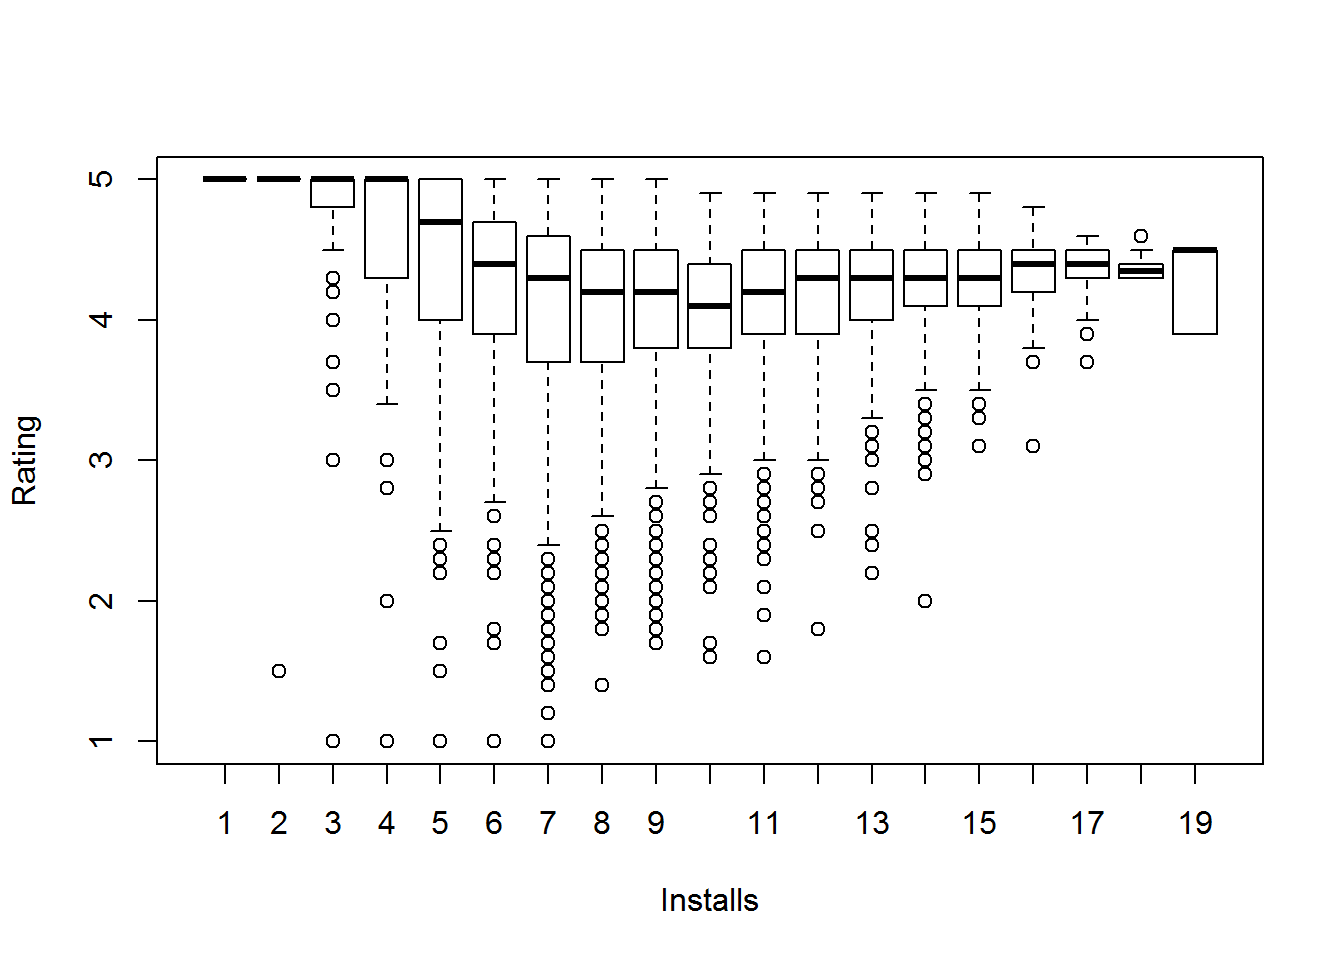
\includegraphics{Lab1_UNI_files/figure-latex/unnamed-chunk-4-1.pdf}

\begin{enumerate}
\def\labelenumi{\arabic{enumi})}
\setcounter{enumi}{2}
\tightlist
\item
  Repeat question (1) except change the number of draws to 10, 1000,
  10,000, and 100,000 storing the results in vectors called
  \textbf{normal10}, \textbf{normal1000}, \textbf{normal10000},
  \textbf{normal100000}.
\end{enumerate}

\begin{Shaded}
\begin{Highlighting}[]
\CommentTok{# Generate 10, 1000, 10,000, and 100,000 random draws from the standard normal distribution}
\NormalTok{normal10 <-}\StringTok{ }\KeywordTok{rnorm}\NormalTok{(}\DataTypeTok{n =} \DecValTok{10}\NormalTok{, }\DataTypeTok{mean =} \DecValTok{0}\NormalTok{, }\DataTypeTok{sd =} \DecValTok{1}\NormalTok{)}
\NormalTok{normal1000 <-}\StringTok{ }\KeywordTok{rnorm}\NormalTok{(}\DataTypeTok{n =} \DecValTok{1000}\NormalTok{, }\DataTypeTok{mean =} \DecValTok{0}\NormalTok{, }\DataTypeTok{sd =} \DecValTok{1}\NormalTok{)}
\NormalTok{normal10000 <-}\StringTok{ }\KeywordTok{rnorm}\NormalTok{(}\DataTypeTok{n =} \DecValTok{10000}\NormalTok{, }\DataTypeTok{mean =} \DecValTok{0}\NormalTok{, }\DataTypeTok{sd =} \DecValTok{1}\NormalTok{)}
\NormalTok{normal100000 <-}\StringTok{ }\KeywordTok{rnorm}\NormalTok{(}\DataTypeTok{n =} \DecValTok{100000}\NormalTok{, }\DataTypeTok{mean =} \DecValTok{0}\NormalTok{, }\DataTypeTok{sd =} \DecValTok{1}\NormalTok{)}
\end{Highlighting}
\end{Shaded}

\begin{enumerate}
\def\labelenumi{\arabic{enumi})}
\setcounter{enumi}{3}
\tightlist
\item
  We want to compare the means of our four random draws. Create a vector
  called \textbf{sample\_means} that has as its first element the mean
  of \textbf{normal10}, its second element the mean of
  \textbf{normal100}, its third element the mean of \textbf{normal1000},
  its fourth element the mean of \textbf{normal10000}, and its fifth
  element the mean of \textbf{normal100000}. After you have created the
  \textbf{sample\_means} vector, print the contents of the vector and
  use the \textbf{length()} function to find the length of this vector.
  (it should be five). There are, of course, multiple ways to create
  this vector. Finally, explain in words the pattern we are seeing with
  the means in the \textbf{sample\_means} vector.
\end{enumerate}

\begin{Shaded}
\begin{Highlighting}[]
\NormalTok{## Sample distribution of the sample mean}
\CommentTok{# library(purrr)}
\NormalTok{sample_means <-}\StringTok{ }\KeywordTok{c}\NormalTok{(}\KeywordTok{mean}\NormalTok{(normal10), }\KeywordTok{mean}\NormalTok{(normal100), }\KeywordTok{mean}\NormalTok{(normal1000), }\KeywordTok{mean}\NormalTok{(normal10000), }\KeywordTok{mean}\NormalTok{(normal100000))}
\KeywordTok{cat}\NormalTok{(}\StringTok{"The content of the sample_means is "}\NormalTok{, sample_means, }\DataTypeTok{seq =} \StringTok{'}\CharTok{\textbackslash{}n}\StringTok{'}\NormalTok{)}
\end{Highlighting}
\end{Shaded}

\begin{verbatim}
## The content of the sample_means is  0.4937354 0.08256659 -0.02687572 -0.006719807 -0.001114476
\end{verbatim}

\begin{Shaded}
\begin{Highlighting}[]
\KeywordTok{cat}\NormalTok{(}\StringTok{"The length of the sample_means is "}\NormalTok{, }\KeywordTok{length}\NormalTok{(sample_means))}
\end{Highlighting}
\end{Shaded}

\begin{verbatim}
## The length of the sample_means is  5
\end{verbatim}

\begin{Shaded}
\begin{Highlighting}[]
\CommentTok{# Answer: the means become closer to 0 as the sample size increasing}
\end{Highlighting}
\end{Shaded}

\begin{enumerate}
\def\labelenumi{\arabic{enumi})}
\setcounter{enumi}{4}
\tightlist
\item
  Let's push this a little farther. Generate 1 million random draws from
  a normal distribution with \(\mu = 3\) and \(\sigma^2 = 4\) and save
  them in a vector named \textbf{normal1mil}. Calculate the mean and
  standard deviation of \textbf{normal1mil}.
\end{enumerate}

\begin{Shaded}
\begin{Highlighting}[]
\NormalTok{normal1mil =}\StringTok{ }\KeywordTok{rnorm}\NormalTok{(}\DecValTok{1000000}\NormalTok{, }\DataTypeTok{mean =} \DecValTok{3}\NormalTok{, }\DataTypeTok{sd =} \DecValTok{4}\NormalTok{)}
\NormalTok{normal1mil_mean =}\StringTok{ }\KeywordTok{mean}\NormalTok{(normal1mil)}
\NormalTok{normal1mil_sd =}\StringTok{ }\KeywordTok{sd}\NormalTok{(normal1mil)}
\KeywordTok{cat}\NormalTok{(}\StringTok{'The mean is'}\NormalTok{, normal1mil_mean, }\StringTok{'}\CharTok{\textbackslash{}n}\StringTok{The std is '}\NormalTok{, normal1mil_sd)}
\end{Highlighting}
\end{Shaded}

\begin{verbatim}
## The mean is 3.000482 
## The std is  3.999923
\end{verbatim}

\begin{enumerate}
\def\labelenumi{\arabic{enumi})}
\setcounter{enumi}{5}
\tightlist
\item
  Find the mean of all the entries in \textbf{normal1mil} that are
  greater than 3. You may want to generate a new vector first which
  identifies the elements that fit the criteria.
\end{enumerate}

\begin{Shaded}
\begin{Highlighting}[]
\NormalTok{new_normal1mil <-}\StringTok{ }\NormalTok{normal1mil}
\NormalTok{new_normal1mil <-}\StringTok{ }\NormalTok{new_normal1mil[new_normal1mil }\OperatorTok{>}\StringTok{ }\DecValTok{3}\NormalTok{]}
\KeywordTok{cat}\NormalTok{(}\StringTok{"the mean of all the entries that are greater than 3 is "}\NormalTok{, }\KeywordTok{mean}\NormalTok{(new_normal1mil))}
\end{Highlighting}
\end{Shaded}

\begin{verbatim}
## the mean of all the entries that are greater than 3 is  6.192317
\end{verbatim}

\begin{enumerate}
\def\labelenumi{\arabic{enumi})}
\setcounter{enumi}{6}
\tightlist
\item
  Create a matrix \textbf{normal1mil\_mat} from the vector
  \textbf{normal1mil} that has 10,000 columns (and therefore should have
  100 rows).
\end{enumerate}

\begin{Shaded}
\begin{Highlighting}[]
\NormalTok{normal1mil_mat =}\StringTok{ }\KeywordTok{matrix}\NormalTok{(normal1mil, }\DataTypeTok{nrow =} \DecValTok{100}\NormalTok{, }\DataTypeTok{ncol =} \DecValTok{10000}\NormalTok{)}
\end{Highlighting}
\end{Shaded}

\begin{enumerate}
\def\labelenumi{\arabic{enumi})}
\setcounter{enumi}{7}
\tightlist
\item
  Calculate the mean of the \(1234^{th}\) column.
\end{enumerate}

\begin{Shaded}
\begin{Highlighting}[]
\NormalTok{mean_col1234 =}\StringTok{ }\KeywordTok{mean}\NormalTok{(normal1mil_mat[,}\DecValTok{1234}\NormalTok{])}
\KeywordTok{cat}\NormalTok{(}\StringTok{"the mean of the $1234^\{th\}$ column is "}\NormalTok{, mean_col1234)}
\end{Highlighting}
\end{Shaded}

\begin{verbatim}
## the mean of the $1234^{th}$ column is  3.113089
\end{verbatim}

\begin{enumerate}
\def\labelenumi{\arabic{enumi})}
\setcounter{enumi}{8}
\tightlist
\item
  Use the \textbf{colSums()} functions to calculate the \emph{means} of
  each column of \textbf{normal1mil\_mat}. Remember, \textbf{?colSums}
  will give you help documents about this function. Save the vector of
  column means with an appropriate name as it will be used in the next
  task.
\end{enumerate}

\begin{Shaded}
\begin{Highlighting}[]
\CommentTok{# normal1mil_colmean = colSums(normal1mil_mat)/100}
\NormalTok{normal1mil_colmean =}\StringTok{ }\KeywordTok{colMeans}\NormalTok{(normal1mil_mat)}
\end{Highlighting}
\end{Shaded}

\begin{enumerate}
\def\labelenumi{\arabic{enumi})}
\setcounter{enumi}{9}
\tightlist
\item
  Finally, produce a histogram of the column means you calculated in
  task (9). What is the distribution that this histogram approximates
  (i.e.~what is the distribution of the sample mean in this case)?
\end{enumerate}

\begin{Shaded}
\begin{Highlighting}[]
\KeywordTok{hist}\NormalTok{(normal1mil_colmean, }\DataTypeTok{col =} \StringTok{'black'}\NormalTok{)}
\end{Highlighting}
\end{Shaded}

\includegraphics{Lab1_UNI_files/figure-latex/unnamed-chunk-12-1.pdf}

\begin{Shaded}
\begin{Highlighting}[]
\CommentTok{# Answer: Based on the shape of histogram, we could draw a conclusion that the normal1mil_colmean follows the normal distribution}
\end{Highlighting}
\end{Shaded}


\end{document}
